
This is the first in a series of tutorials on the use of the \eass\ variant of the \gwendolen\ language that was first developed as part of the Engineering Autonomous Space Software project.  The \eass\ variant is adapted for use with physical systems and simulations, such as mobile robots, satellites and unmanned aircraft.  This tutorial covers the basic concepts behind the \eass\ variant and its differences to the \gwendolen\ language.  

Files for this tutorial can be found in the \texttt{mcapl} distribution in the directory 
\begin{quote}
\texttt{src/examples/eass/tutorials/tutorial1}.
\end{quote}

The tutorial assumes familiarity with the \gwendolen\ programming language.

\section{Abstraction and Reasoning Engines}

\begin{figure}[htb]
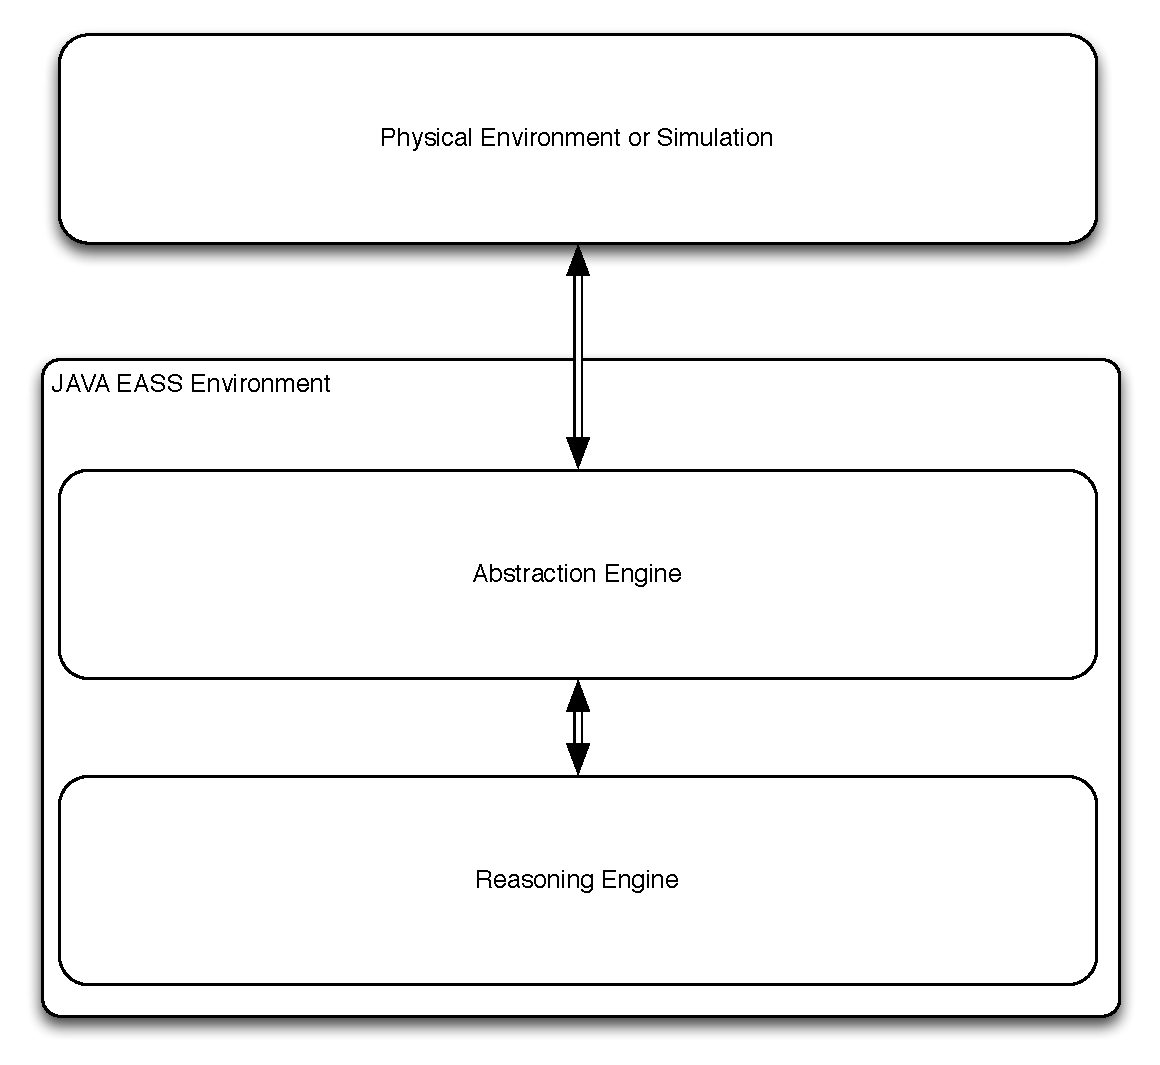
\includegraphics[width=\textwidth]{images/arch.pdf}
\caption{The Architecture of an \eass\ Agent}
\label{fig:arch}
\end{figure}
Figure~\ref{fig:arch} shows the typical architecture of an \eass\ Agent.  The agent is actually a pair of agents, the \emph{reasoning engine} which is responsible for complicated reasoning tasks, and the \emph{abstraction engine} which is responsible for processing and filtering incoming perceptions so only those actually needed for reasoning are passed on to the reasoning engine itself.

The reasons for this separation are primarily driven by the observation that BDI agents are unable to process incoming perceptions from real or simulated sources fast enough and so they get ``clogged'' by an ever increasing number of intentions to do with perception processing.  

The theoretical underpinnings of this architecture are described in~\cite{DALT10:abstraction,Dennis2016}.  The key points are that the \emph{reasoning engine} does not interact with the physical world (or a simulation) at all.  It gains perceptions via \emph{shared beliefs} which are communicated with the abstraction engine via the Java \eass\ environment.  Similarly most of its actions (ideally all) are communicated to the abstraction engine which then reifies them (e.g., adding more low level detail that may be required by the physical system or simulation to actually enact the action).  As a rule of thumb while perceptions and actions, as used by the physical system or simulation generally involve numeric values, reasoning generally uses logical (``yes/no'') information and outputs simple non-numeric commands.  Therefore the abstraction engine should be responsible for converting numeric data (``distance = 5.4m'') into logical statements (``too close'') and converting simple commands (``slow down'') into numerical instructions (``apply a deceleration of $-1m/s^2$'').  This is only a rule of thumb and the reality is that a certain amount of experimentation is often required to balance a system appropriately so that reasoning happens fast enough to adequately control the physical system.

In order for this to work \gwendolen's reasoning cycle was adapted slightly, a set of dedicated actions were introduced for handling shared beliefs and delegated actions, and some new constructs were added to the language.

\section{Key Differences}
\subsection{Perception Processing}
In the \gwendolen\ language incoming perceptions are converted into intentions which contain a deed to add the perception to the belief base.  In theory this gives the agent more control over the contents of its beliefs (although in practice no use has ever been made of this).  However a side effect is that it takes the agent two turns of the reasoning cycle to convert a perception into a belief and this slowed down the processing of perceptions.

In the \eass\ variant, therefore, new perceptions are placed directly into the agent's belief base during the perception stage of the reasoning cycle.

\subsection{Identifying Abstraction and Reasoning Engines}
Since each agent is, in fact, a pair of agents, it is necessary to identify and link the abstraction and reasoning engines.  This is done by starting the abstraction engine with the line
\begin{verbatim}
:abstraction: agentname
\end{verbatim} 
instead of 
\begin{verbatim}
:name: agentname
\end{verbatim} 
which is reserved as the start of the reasoning engine code.  So long as the two agents have the same name then the environment will link them.

\subsection{Shared Beliefs}
The reasoning engine does not receive percepts from the outside world but only via a \emph{shared belief} set.  An abstraction engine may get perceptions both form the outside world and from the shared beliefs.

\eass\ environments support this communication via support for two dedicated actions, \lstinline{assert_shared(B)} and \lstinline{remove_shared(B)} which can be used to assert and remove the shared belief, \lstinline{B}.

Both the abstraction and reasoning engine may use these commands.

\subsection{Perf}
The reasoning engine may also request the abstraction engine to reify an action to be sent to some external system.  It does this via the dedicated actions, \texttt{perf}.  This sends a message to the abstraction engine asking it to adopt a perform goal.

This means that abstraction engines need to implement plans for handling perform messages.

\section{Example}
Example~\ref{code:EASSexample} shows a simple \eass\ program to control a car by making it accelerate up to the speed limit and then maintain that speed.  Lines 3-28 are the abstraction engine, and lines 30-46 are the reasoning engine.

\begin{ourexample}
\label{code:EASSexample} \quad \\
\begin{lstlisting}[basicstyle=\sffamily,style=easslisting,language=Gwendolen]
EASS

:abstraction: car

:Initial Beliefs:

speed_limit(5)
											
:Initial Goals:
		
:Plans: 
/* Default plans for handling messages */
+.received(:tell, B): {True} <- +B;   
+.received(:perform, G): {True} <- +!G [perform];
+.received(:achieve, G): {True} <- +!G [achieve];

+started : {True} <-
	assert_shared(start);

+yspeed(X) : {B speed_limit(SL), SL < X} <-
	assert_shared(at_speed_limit);
+yspeed(X) : {B speed_limit(SL), X < SL} <-
	remove_shared(at_speed_limit);
	
+! accelerate [perform] : {B yspeed(X)} <- accelerate;
+! accelerate [perform] : {~B yspeed(X)} <- 
     print("Waiting for Simulator to Start");
+! maintain_speed [perform] : {True} <- maintain_speed;

:name: car
			
:Initial Beliefs:
													
:Initial Goals:
		
:Plans: 

+start: {True} <-
	+!at_speed_limit[achieve];

+! at_speed_limit [achieve] : {True} <-
	perf(accelerate),
  *at_speed_limit;

+at_speed_limit: {True} <-
	perf(maintain_speed);
\end{lstlisting}
\end{ourexample}

As an initial belief the abstraction engine has that the speed limit on the road is 5.  Every time the perception, \lstinline{yspeed(X)} comes in (lines 20-23) the abstraction compares this to the speed limit and, if appropriate asserts a shared belief (NB., we are using $+_{\Sigma}(B)$ as shorthand for \lstinline{assert_shared(B)} and  $-_{\Sigma}(B)$ as shorthand for \lstinline{remove_shared(B)} ).

Lines 13-15 are the standard plans for handling messages.  It is important that the abstraction engine has these to it correctly handles \texttt{perf} requests from the reasoning engine.

If the reasoning engine has a goal to reach the speed limit (lines 41-43) then it requests the abstraction engine to perform \lstinline{accelerate}.  This is passed on directly to the environment (line 25).  Once the reasoning engine believes the speed limit is reached (lines 45 and 46) then it requests the abstraction engine to perform \lstinline{maintain_speed}.

Lastly, in order to allow time for the simulation to start, a perception, \lstinline{started} is used.  When the abstraction engine perceives this (lines 17 and 18) it asserts the shared belief \lstinline{start} which causes the reasoning engine to adopt the goal of reaching the speed limit (lines 38 and 39).

The environment passes on requests for acceleration etc., to the simulator and reports on the simulated speed and position using perceptions.

\subsection{Running the Example}

The example uses \texttt{MotorwayMain} which you can find in the directory \texttt{src/examples/eass/tutorials/motorwaysim}.  This must be run as a separate java program and must be started before the \eass\ program is run.  When it starts you should see message:

\begin{verbatim}
Motorway Sim waiting Socket Connection
\end{verbatim}

Now run the \eass\ program as normal for \ail\ programs.  You will find the \ail\ configuration file in the tutorial directory.  You should see the window shown in figure~\ref{fig:motorwaysim} (NB.  You may need to move other windows out of the way to find it!).  Click on start and you should see the car accelerate up to a speed of 5.

\begin{figure}
\begin{center}
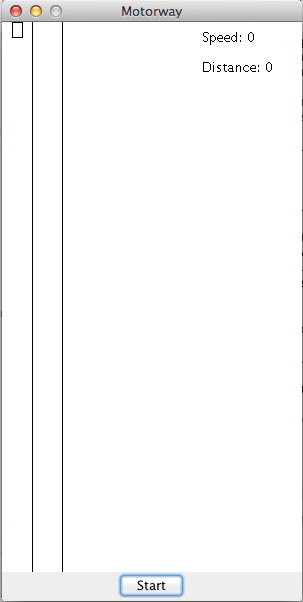
\includegraphics[width=2in]{images/EASSmotorwaysim.png}
\end{center}
\caption{The Motorway Simulator}
\label{fig:motorwaysim}
\end{figure}

\section{Exercise}

\texttt{eass.tutorials.tutorial1.CarOnMotorwayEnvironment} provides four actions to the abstraction engine.
\begin{description}
\item[accelerate] Accelerates the car.
\item[decelerate] Decelerates the car (if the car reaches a speed of 0 it stops).
\item[maintain\_speed] Maintains the speed of the car.
\item[calculate\_totaldistance(D)] unifies \texttt{D} with the total distance the car has travelled.
\end{description}

The perceptions it sends to the abstraction engine are:
\begin{description}
\item[xpos(X)] \texttt{X} is the x position of the car.
\item[ypos(X)] \texttt{X} is the y position of the car.
\item[xspeed(X)] \texttt{X} is the speed of the car in the x direction.
\item[yspeed(X)] \texttt{X} is the  speed of the car in the x direction.
\item[started] The simulation has started.
\end{description}
The x and y positions of the car reset to 0 each time the car loops around the simulator window.

\subsection{Exercise 1}
Adapt \texttt{car.eass} so that the reasoning engine prints out the total distance travelled when it reaches the speed limit.

\subsection{Exercise 2}
Extend \texttt{car.eass} so that it accelerates to the speed limit, then continues until it has reached a total distance of 600 metres and then decelerates.  

Hint. The solution does this by having the reasoning engine request an alert at 600 units.  The abstraction engine then calculates the total distance each time \texttt{ypos} updates until this is reached at which point it alerts the reasoning engine.  There are lots of other ways to do this but this solution maintains the idea that the reasoning engine makes decisions while the abstraction engine processes data.  

\begin{sloppypar}
Sample answers for the exercises can be found in \texttt{eass/examples/tutorials/tutorial1/answers}.
\end{sloppypar}

